\section{Beweiserschnittstelle}%

Die Beweiserschnittstelle lässt Worthwhile-""Programm"-spezifikationen
und prädikatenlogische Formeln mit Kontext von einem Beweiser
überprüfen. Der Formelkontext kann zum Beispiel einem
Ausführungszustand entsprechen, sodass eine Programm"-spezifikation
auch nur für konkrete statt für alle Programmdurchläufe geprüft werden
kann. Das dem Aufrufer zurückgelieferte Überprüfungsergebnis besteht
unter anderem aus der Programm"-spezifikations-"" bzw.\
Formelvalidität.

In den folgenden Abschnitten wird zunächst das Format der Eingaben,
anschließend deren Vorbereitung für einen Beweiseraufruf und zuletzt
die Ergebniserstellung aus der Beweiserausgabe beschrieben.%

\subsection{Eingabedaten}%

\subsubsection{Worthwhile-""Programm"-spezifikation}%

Die Programm"-spezifikation wird dem Abstract-""Syntax-""Tree~(AST)
entnommen, welcher aus einem Worthwhile-""Text erstellt wurde. Sie
setzt sich aus dem WHILE-""Programmtext und den Annotationen
zusammen.%

Siehe \type{AST::Program}%

Siehe \texttt{SpecificationChecker::checkProgram}%

\subsubsection{Prädikatenlogische Formel mit Kontext}%

Die Formel wird einem AST entnommen, dessen Wurzelknoten ein
Worthwhile-""Ausdruck ist. Insbesondere ist unbekannt, wo die Formel
in einem Programmtext steht oder wie ihre Validität verwendet wird.
Den Kontext geben eine Abbildung von Variablen auf Bedeutungen
und eine Axiomliste an.%

Siehe \type{AST::Expression}%

Siehe \texttt{SpecificationChecker::checkAnnotation}%

\subsection{Vorbereitungen für einen Beweiseraufruf}%

In den folgenden Unterabschnitten werden die Vorbereitungen der
Beweiserschnittstelle an den Eingabedaten, bevor diese an den
Beweiser übergeben werden, beschrieben. Die Vorbereitungen
betreffen Worthwhile-spezifische Syntax und Semantik.%

\subsubsection{Axiome}%

Axiome werden als Annahmen behandelt, die für die gesamte
Spezifikation bzw.\ Formel gelten.%

\subsubsection{Funktionsdefinition}%

Funktionen werden modular spezifiziert und überprüft. Ihre
Spezifikation besteht sowohl aus Annahmen über die Aktualparameter
eines Funktionsaufrufs als auch aus Zusicherungen, welche für den
Rückgabewert gelten müssen. Die Annahmen werden Vorbedingungen
genannt und gelten als solche für den gesamten Funktionskörper. Die
Zusicherungen heißen auch Nachbedingungen und bilden zusammen mit den
Vorbedingungen den Funktionsvertrag.%

Im AST werden \texttt{requires}-Knoten als Vorbedingungen und
\texttt{ensures}-Knoten als Nachbedingungen interpretiert.%

Siehe \texttt{FP020}%

\subsubsection{Funktionsaufruf}%

Für jeden Funktionsaufruf in der Spezifikation bzw.\ Formel gilt die
Validität des jeweiligen Funktionsvertrags als Annahme. Insbesondere
wird der Funktionskörper nicht betrachet.%

\subsubsection{Arrayzugriff}%

Für jeden Arrayzugriff in der Spezifikation bzw.\ Formel gelten die
drei Axiome (A1), (A2) und (A3) als Annahmen \footnote{Die Axiome sind
der Theorie
\url{http://goedel.cs.uiowa.edu/smtlib/theories/ArraysEx.smt2}
entnommen}. Hierbei ist $\mathbb{A}$ eine Indexmenge, $\mathbb{B}$
eine Basismenge sowie $\mathbb{B}^\mathbb{A}$ die Menge aller Arrays
mit der Indexmenge $\mathbb{A}$ und der Basismenge $\mathbb{B}$. %

\begin{description}%
    \item[(A1)] \begin{math}\forall i \in \mathbb{A}, e \in \mathbb{B} : \{\texttt{true}\} a[i] := e \{a[i] = e\}\end{math}%
    \item[(A2)] \begin{math}\forall i, j \in \mathbb{A}, e, f \in \mathbb{B} : \{i \neq j \wedge a[i] = e\} a[j] := f \{a[i] = e\}\end{math}%
    \item[(A3)] \begin{math}\forall a, b \in \mathbb{B}^\mathbb{A} : (\forall i, j \in \mathbb{A} : a[i] = b[j]) \Rightarrow a = b\end{math}%
\end{description}%

Außerdem muss vor jedem Arrayzugriff in der Spezifikation bzw.\ Formel
als Zusicherung gelten, dass der Feldindex des Zugriffs nicht negativ
und echt kleiner als die Deklarationsgröße des Arrays ist. Damit wird
erstens erreicht, dass ein Programmdurchlauf, der einen ungültigen
Arrayzugriff enthält und deswegen entweder gar nicht oder mit
undefiniertem Ergebnis terminiert, für eine valide Spezifikation
ausgeschlossen ist, und zweitens, dass die Validität der Spezifikation
bzw.\ Formel bei ungültigem Feldzugriff unabhängig vom Beweiser
festgelegt ist.%

\subsubsection{Division}%

Vor jeder Division in der Spezifikation bzw.\ Formel muss als
Zusicherung gelten, dass der Dividend ungleich Null ist. Damit wird
erstens erreicht, dass ein Programmdurchlauf, der eine Division durch
Null enthält und deswegen entweder gar nicht oder mit undefiniertem
Ergebnis terminiert, für eine valide Spezifikation ausgeschlossen ist,
und zweitens, dass die Validität der Spezifikation bzw.\ Formel bei
Division durch Null unabhängig vom Beweiser festgelegt ist.%

\subsubsection{Variablendeklarierung}%

Wird eine Variable ohne Initialisierung deklariert, gilt für den
nachfolgenden Spezifikationsteil eine Initialisierung der Variablen
mit dem Standardwert Null für \int- und \texttt{false} für
\bool-""Variablen sowie dem jeweiligen Standardwert des
Basistyps für Array-""Variablen als Annahme.%

\subsubsection{Typprüfung}%

Die in Worthwhile vorhandenen Datentypen \int{} und
\bool{} werden beide vom Beweiser ohne Typkonvertierung
unterstützt. Die Typen von Sprachelementen werden bei Parameterangabe,
Variablenreferenz und Variablendefinition in der Eingabe vom Beweiser
geprüft. Treten in einem dieser Fälle nicht übereinstimmende Typen
auf, liefert der Beweiser einen Typfehler in der Ausgabe und diese ist
im zurückgelieferten Überprüfungsergebnis enthalten.%

\subsubsection{Prädikatenlogische Formel}%

Die prädikatenlogische Formel wird so behandelt, dass sie als
Zusicherung gelten muss.%

\subsubsection{Abbildung von Variablen auf Bedeutungen}%

Die Abbildung wird so behandelt, dass in der gesamten Formel die
Annahme gilt, dass die Variablen die angegebenen Bedeutungen haben.%

\subsection{Ausgabedaten}%

\subsubsection{Validität}%

Die Validität der Spezifikation bzw.\ Formel ist entweder
bewiesenermaßen gegeben, verifizierbar nicht gegeben oder unbekannt.
Ist der Beweiser zu einem Ergebnis gekommen, ist die Spezifikation
genau dann valide, wenn bewiesen wurde, dass jeder mögliche
Programmdurchlauf niemals den Annahmen widerspricht und die
Zusicherungen an ihrer Position in der Spezifikation erfüllt. Die
Formel ist genau dann valide, wenn bewiesen wurde, dass es keine
Belegung der Variabeln in der Formel gibt, sodass die Formel nicht
gültig ist, d.~h.\ zu \texttt{false} ausgewertet wird. Wenn der
Beweiser zu keinem Ergebnis gekommen ist, wird die Validität der
Spezifikation bzw.\ Formel im Überprüfungsergebnis als unbekannt
angegeben.%

\subsubsection{Beweiserausgabe}%

Die komplette Ausgabe des Beweisers wird zur Fehleruntersuchung in das
Überprüfungsergebnis aufgenommen. Sie kann zur Ergebnisverifikation
neben Typfehlern ein Modell für Variablen in der von der
Beweiserschnittstelle erstellten Formel enthalten, wenn die
Spezifikation bzw.\ die Formel nicht valide ist, d.~h.\ ein
Programmdurchlauf bzw.\ eine Variablenbelegung existiert, sodass einer
Annahme widersprochen wird oder eine Zusicherung nicht erfüllt ist
bzw.\ die Formel zu \texttt{false} ausgewertet wird. Es findet
insbesondere keine Interpretation der Beweiserausgabe durch die
Beweiserschnittstelle, welche zum Beispiel aufgrund eines Modell eine
Abbildung von Variablen auf Belegungen festlegen könnte, statt.%

% TODO Klassenentwurf

\begin{figure}[ph]%

    \caption{Klassendiagramm der Komponente Beweiserschnittstelle mit
    der Schnittstellenklasse \type{SpecificationChecker}}%

    \hspace{-33mm}%
    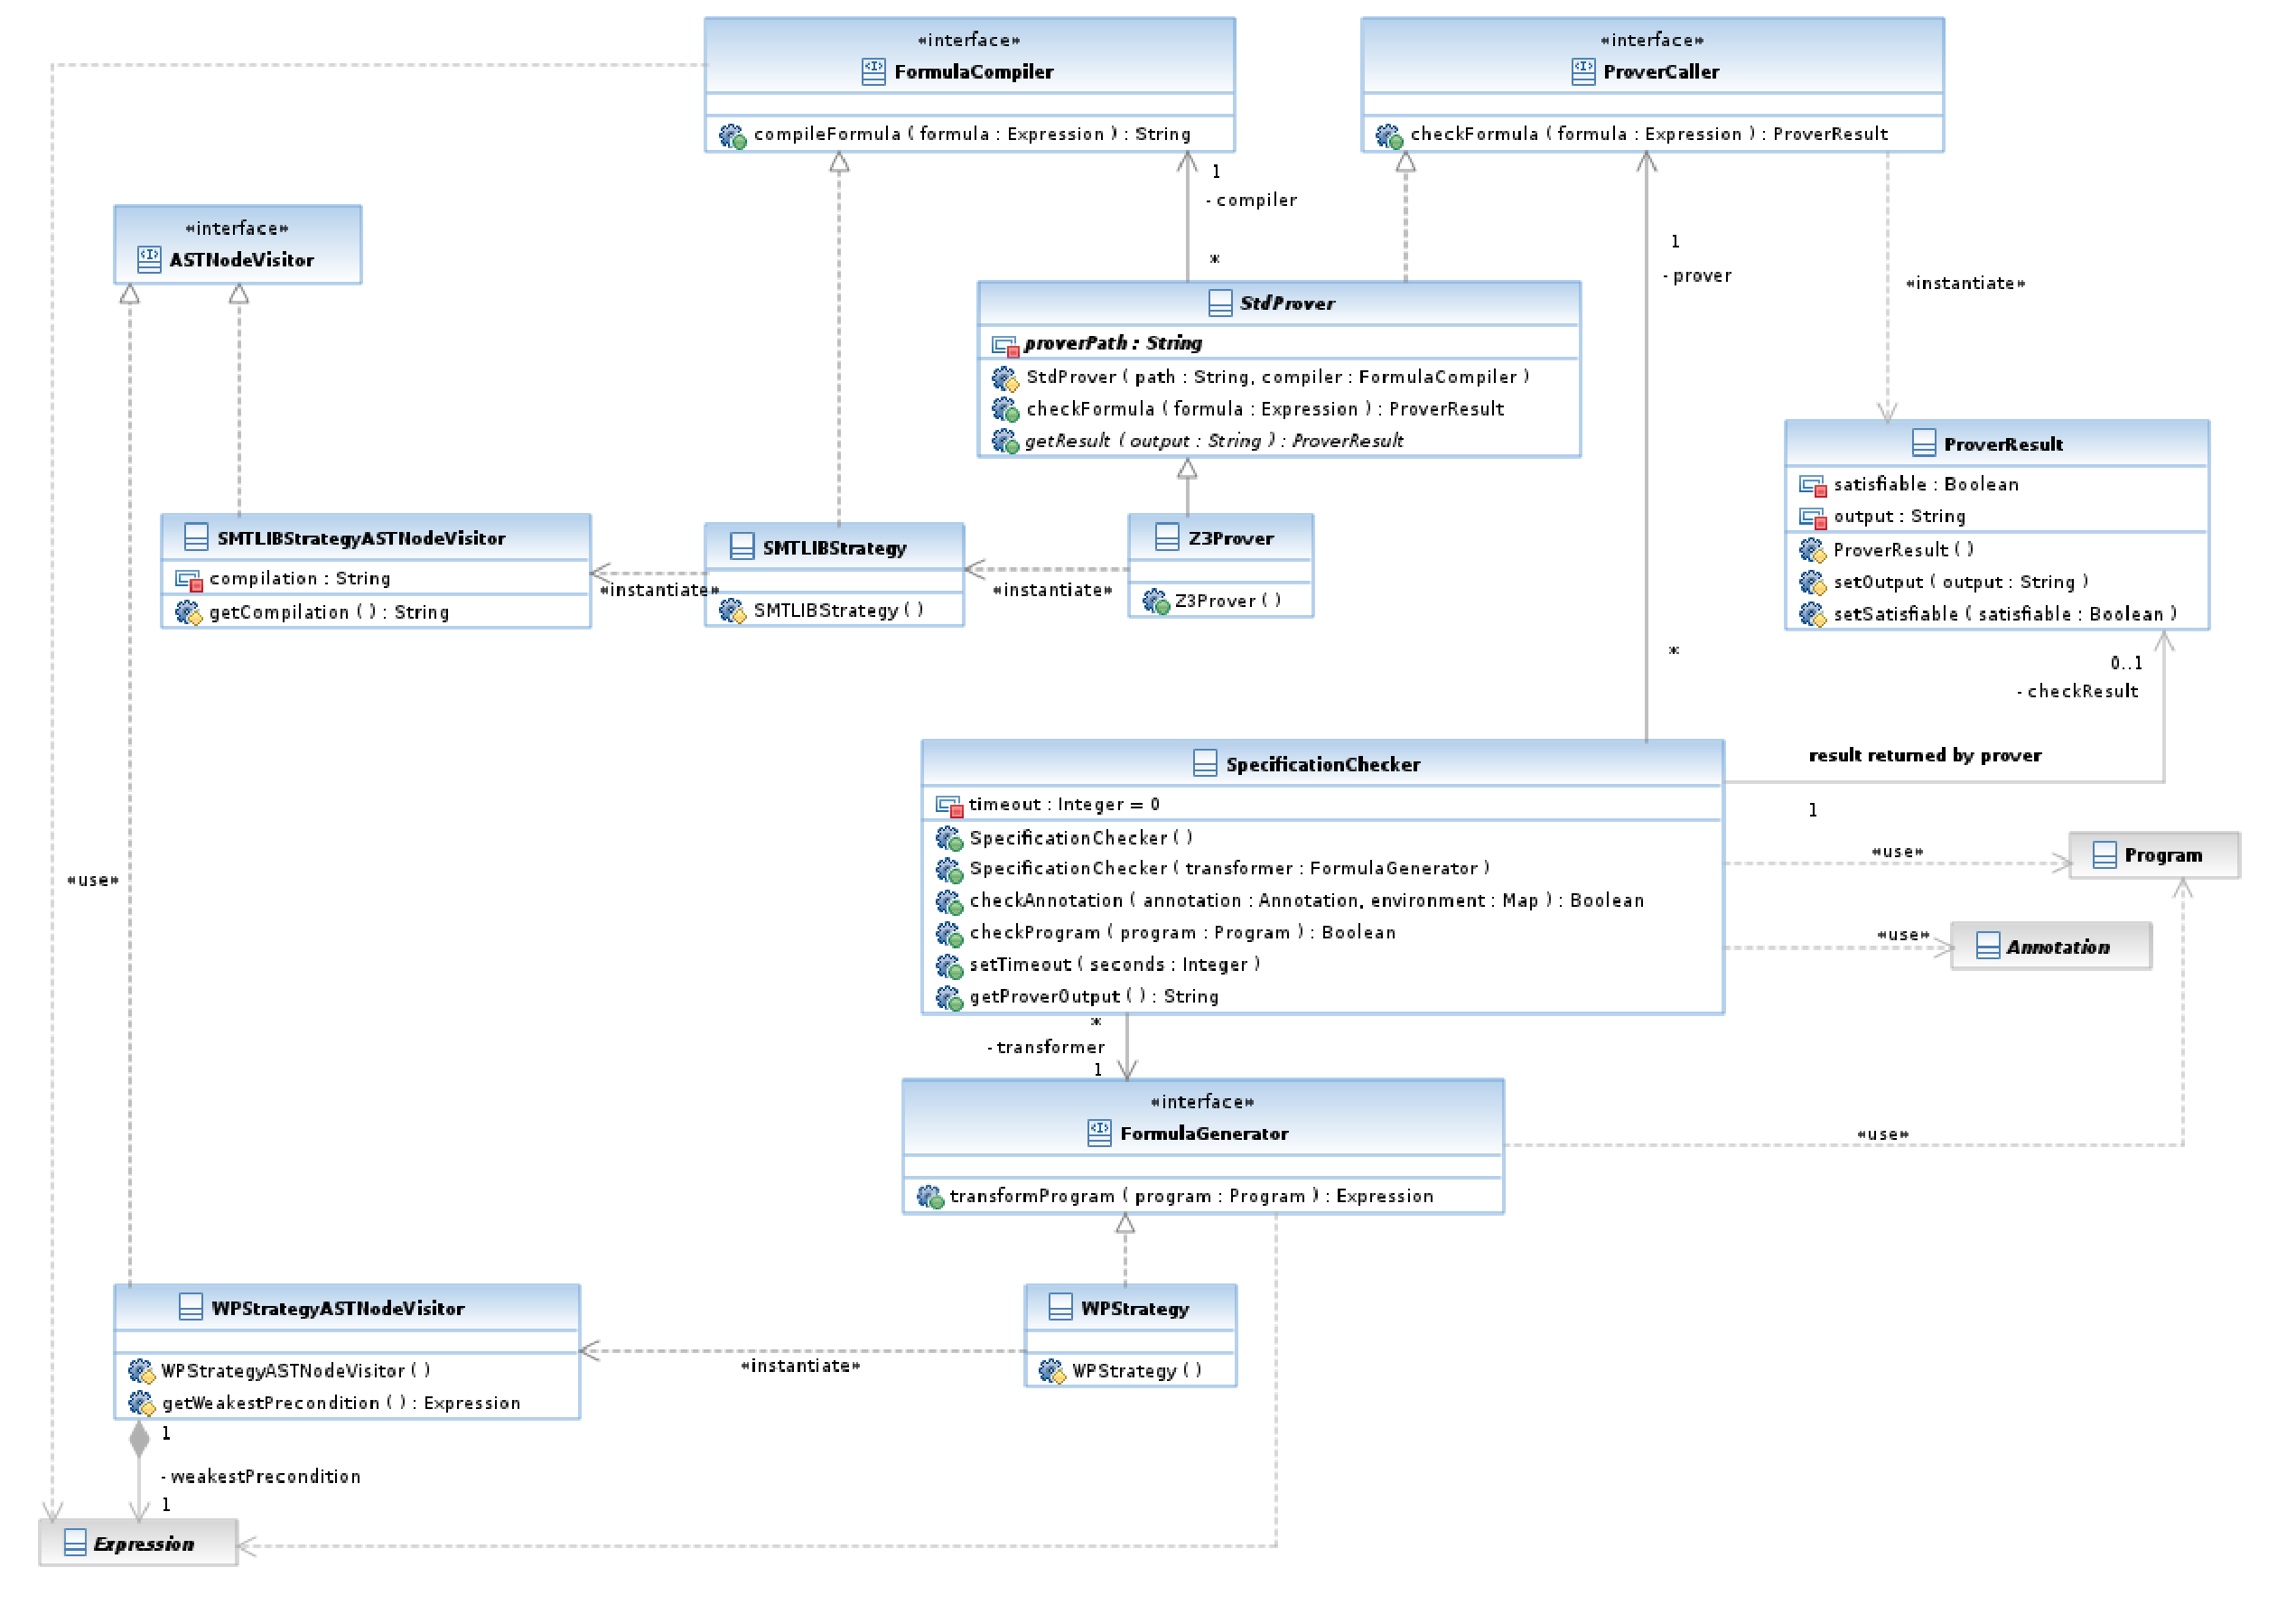
\includegraphics[width=1.4\textwidth]{diagrams/prover_component.pdf}%
    \label{prover_classdiagram}%
\end{figure}%

\subsection{package Prover}%

In Abbildung~\ref{prover_classdiagram} ist der Klassenentwurf der
Beweiserschnittstelle, wie er im Folgenden ausformuliert ist, zur
Übersicht als UML-""Klassendiagramm mit Vererbungs-"" und
Assoziations"-beziehungen dargestellt.%

\subsubsection{enumeration Validity}%

Gibt an, ob die überprüfte Spezifikation bzw.\ Formel valide ist oder
dass die Validität nicht bestimmt werden konnte. Aufgrund der
Komplexität von Spezifikation und Beweis"-findung können Überprüfungen
in allen drei Zuständen enden und reichen die beiden Zustände
\texttt{VALID} und \texttt{INVALID} nicht aus.%

\begin{description}%
    \literal{VALID}%

    Bedeutet, dass für alle Programm"-durchläufe die Spezifikation
    bzw.\ für alle Belegungen die Formel erfüllt ist.%

    \literal{INVALID}%

    Bedeutet, dass es Programm"-durchläufe bzw.\ Belegungen gibt,
    sodass die Spezifikation bzw.\ Formel nicht erfüllt ist.%

    \literal{UNKNOWN}%

    Bedeutet, dass unbekannt ist, ob nicht erfüllende
    Programm"-durchläufe bzw.\ Belegungen existieren.%

\end{description}%

\subsubsection{class SpecificationChecker}%

Ist Fassaden"-klasse für die Komponente Beweiserschnittstelle. Zur
Überprüfung einer Spezifikation bzw.\ Formel arbeitet sie dreistufig
und benutzt dazu die allgemeineren Funktionsklassen der Komponente.
Sowohl in der ersten als auch in der letzten Stufe fungiert die Klasse
außerdem als Adapter, da für Worthwhile-""Programme spezifische Syntax
und Semantik existiert und sich das Beweiserergebnis nicht unmittelbar
auf das übergebene Worthwhile-""Programm, sondern auf die daraus
erstellte Formel, bezieht.%

\begin{enumerate}%

    \item Übersetzung Worthwhile-""spezifischer
    Syntax~(Funktions"-verträge, Axiome) und Ergänzung spezifischer
    Semantik~(Array"-zugriff, Division, Standard"-werte) in der
    Spezifikation~(\texttt{program}) bzw.\
    Formel~(\texttt{annotation})%

    \item Anwendung der Transformationen eines Kalküls zur
    Programm"-verifikation, das die Spezifikation bzw.\ Formel in eine
    prädikatenlogische Formel vom Typ \type{AST::Expression}
    überführt. Diese Stufe ist in einem Aufruf des
    \texttt{transformer}s gekapselt.%

    \item Übersetzung der prädikatenlogischen Formel aus der zweiten
    Stufe in eine Zeichenkette, mit welcher als Eingabe der Beweiser
    ausgeführt wird. Diese Stufe ist in einem Aufruf des
    \texttt{prover}s gekapselt, dessen Rückgabe die zurückgelieferte
    \type{Validity} entnommen wird.%

\end{enumerate}%

In der Implementierungs"-phase sollen typische Aufruf"-szenarien wie
die Verifikation von Schleifeninvarianten identifiziert und
Bequemlichkeitsmethoden dafür erstellt werden, welche der
Beweiserschnittstelle zur Vereinfachung der Benutzung hinzugefügt
werden.%

\begin{description}%
    \attr{private timeout : Integer = 0}%

    Zeit in Sekunden, die ein Beweiser"-aufruf höchstens dauern darf.%

    Siehe \texttt{setTimeout()}%

    \attr{private prover : Theorem"-Prover::Prover"-Caller = Theorem"-Prover::Z3"-Prover()}%

    Beweiser, der zur Prüfung der Validität prädikatenlogischer
    Formeln aufgerufen wird.%

    \attr{private transformer : Program"-Transformer::Formula"-Generator}%

    Programm"-transformator, der zur Erstellung einer zu beweisenden
    prädikatenlogischen Formel aus einer Programm"-spezifikation,
    welche bei Validität die Korrektheit des Programms verifiziert,
    aufgerufen wird.%

    Siehe \texttt{Specification"-Checker()}%

    Siehe \texttt{Specification"-Checker(: Program"-Transformer::Formula"-Generator)}%

    \attr{private check"-Result : Theorem"-Prover::Prover"-Result = null}%

    Ergebnis der letzten Spezifikations-"" bzw.\ Formel"-überprüfung.%

\end{description}%

\begin{description}%
    \method{public Specification"-Checker()}%

    Erstellt einen \type{Specification"-Checker} mit der
    \type{Program"-Transformer::WP"-Strategy} als \texttt{transformer}
    und dem \type{Theorem"-Prover::Z3"-Prover} als \texttt{prover}.%

    \method{public Specification"-Checker(transformer : Program"-Transformer::Formula"-Generator)}%

    Erstellt einen \type{Specification"-Checker}, der
    \texttt{transformer} zur Programm"-transformation und den
    \type{Theorem"-Prover::Z3"-Prover} als \texttt{prover} verwendet.%

    \method{public check"-Program(program : AST::Program) : Validity}

    Überprüft mit Hilfe des \texttt{prover}s die Validität der Spezifikation
    \texttt{program}. Es wird nur dann \texttt{VALID} zurückgeliefert,
    wenn \texttt{program} beweisbar valide ist, \texttt{INVALID} nur
    dann, wenn ein nicht erfüllendes Modell existiert und
    \texttt{UNKNOWN} sonst~(z.~B.\, wenn \texttt{timeout}
    überschritten wurde oder der Beweiser ohne Ergebnis zurückgekehrt
    ist).%

    %Siehe \texttt{getCheckResult()}%

    Siehe \texttt{FP005}%

    \mlmethod{public check"-Annotation(annotation : AST::Annotation,\\
    environment : String"-To"-Value"-Map) : Validity}

    Überprüft mit Hilfe des \texttt{prover}s die Validität der Annotation
    \texttt{annotation}. Es wird nur dann \texttt{VALID}
    zurückgeliefert, wenn \texttt{annotation} im Kontext
    \texttt{environment} beweisbar valide ist, \texttt{INVALID} nur
    dann, wenn ein nicht erfüllendes Modell existiert und
    \texttt{UNKNOWN} sonst~(z.~B.\, wenn \texttt{timeout}
    überschritten wurde oder der Beweiser ohne Ergebnis zurückgekehrt
    ist).%

    %Siehe \texttt{get"-Check"-Result()}%

    Siehe \texttt{FP005}%

    %\method{public get"-Check"-Result() : Theorem"-Prover::Prover"-Result}
    %
    %Liefert für den vorhergehenden Aufruf von %\texttt{check"-Program()}
    %oder \texttt{check"-Annotation()} das Ergebnis des Beweiseraufrufs und
    %\texttt{null}, wenn zuvor weder ein Programm noch eine Annotation
    %überprüft wurde.%

    \method{public set"-Timeout(seconds : Integer)}

    Setzt den Timeout für Aufrufe von \texttt{check"-Program()} und
    \texttt{check"-Annotation()} auf den Wert von \texttt{seconds}.
    Nach Überschreiten des Timeouts wird der Beweiseraufruf
    abgebrochen. Ist der angegebene Wert negativ, wird er als Null
    interpretiert.%

\end{description}%

\subsection{package Prover::TheoremProver}%

\subsubsection{enumeration FormulaSatisfiability}%

Gibt den Ausgang einer Beweiser"-überpüfung, ob eine
prädikatenlogische Formel erfüllbar ist, an oder dass die
Erfüllbarkeit unbekannt ist. Aufgrund der Komplexität von
Beweis"-findungen treten alle drei Zustände auf und genügt kein
\bool-Typ.%

\begin{description}%
    \literal{SATISFIABLE}%

    Es wurde bewiesen, dass eine erfüllende Belegung existiert.%

    \literal{UNSATISFIABLE}%

    Es wurde bewiesen, dass es keine erfüllende Belegung gibt.%

    \literal{UNKNOWN}%

    Es ist unbekannt, ob ein Modell für die prädikatenlogische Formel
    existiert.%

\end{description}%

\subsubsection{class ProverResult}%

Fasst das Überprüfungs"-ergebnis eines Beweiser"-aufrufs zusammen.
Diese Klasse könnte auch die Fehler-"" und Modell"-extraktion aus der
Beweiser"-ausgabe kapseln und über ihre Schnittstelle wie Attribute
verfügbar machen. Dann würde der Konstruktor nur noch mit der
Beweiser"-ausgabe aufgerufen. Zunächst wird aber das
Erfüllbarkeits"-ergebnis von der erstellenden Klasse gesetzt und die
Ausgabe nur der Vollständigkeit halber sowie zur Fehleranalyse
mitangegeben.%

\begin{description}%
    \attr{private output : String}%

    Die vom Beweiser während seiner Ausführung generierte Ausgabe.%

    \attr{private satisfiability : Formula"-Satisfiability}%

    Das der Beweiser"-ausgabe \texttt{output} entnommene
    Erfüllbarkeits"-ergebnis.%

\end{description}%

\begin{description}%
    \method{protected Prover"-Result(satisfiability : Formula"-Satisfiability, output : String)}%

    Erstellt eine einfache Datenstruktur, die das
    Erfüllbarkeits"-ergebnis \texttt{satisfiability} und die
    Beweiserausgabe \texttt{output} bündelt.%

\end{description}%

\subsubsection{interface Formula"-Compiler}%

Implementierungen dieser Schnittstelle übersetzen eine
prädikatenlogische Formel \texttt{formula} vom Typ
\type{AST::Expression} in die Eingabe"-sprache eines Beweisers, sodass
dieser mit der von \texttt{compile"-Formula()} zurückgelieferten
Zeichenkette die Erfüllbarkeit von \texttt{formula} prüfen kann. Die
Abhängigkeit nur von dieser Schnittstelle und nicht von
Implementierungen ermöglicht die Austauschbarkeit von Compilern und
Beweiser"-sprachen~("`Strategien"').%

\begin{description}%
    \method{public compileFormula(formula : AST::Expression) : String}%

    Liefert eine Übersetzung von \texttt{formula} in eine
    Beweiser"-sprache, sodass sich ein erfüllendes Modell eines Beweisers, der
    diese Sprache interpretiert, genau auf ein erfüllendes Modell von
    \texttt{formula} abbilden lässt~(Bedeutungs"-erhalt).%

    %\method{protected Formula uncompileFormula(String formula)}%

\end{description}%

\subsubsection{class SMTLIB"-Strategy}%

\texttt{implements AST::AST"-Node"-Visitor, Formula"-Compiler}%

Ist eine Implementierung der Schnittstelle \type{Formula"-Compiler},
die prädikatenlogische Formeln nach \texttt{SMTLIB} übersetzt.%

Außerdem implementiert die Klasse die Schnittstelle
\type{AST::AST"-Node"-Visitor}, um sich selbst als "`Besucher"' dem
AST-""Teilbaum, dessen Wurzel \texttt{formula} ist, zu übergeben. Der
Zustand des "`Besuchers"' ist die Ausgabe"-zeichenkette und die
Implementierungen der \texttt{visit()}-""Methoden hängen an diese den
dem jeweiligen Knoten entsprechenden \texttt{SMTLIB}-""Funktionsaufruf
an und übergeben den "`Besucher"' an die Kinderknoten, damit diese die
Funktionsparameter belegen. Hierbei wird ausgenutzt, dass die
\texttt{SMTLIB}-""Syntax mit ihrem heftigen Klammergebrauch und der
Präfixschreibweise auch für alle Operatoren Texte baumartig aufbauen
lässt.%

\begin{description}%
    \attr{private compilation : String = ''''}%

    Repräsentiert stets den aktuellen Kompilier"-stand und nach dem
    Rückkehren das fertige Kompilat.%

\end{description}%

\subsubsection{interface Prover"-Caller}%

Implementierungen dieser Schnittstelle kapseln Beweiser"-aufrufe für
gegebene prädikatenlogische Formeln \texttt{formula}. Das Ergebnis
eines Aufrufs wird als \type{Prover"-Result} zurückgegeben. Wie bei
\type{Formula"-Compiler} ermöglicht die Abhängigkeit von nur dieser
Schnittstelle sowohl die Austauschbarkeit des tatsächlich verwendeten
Beweisers als auch des Aufruf"-protokolls~(Bibliotheks"-funktionen,
Programm"-ausführung).%

\begin{description}%
    \method{public check"-Formula(formula : AST::Expression) : Prover"-Result}%

    Ruft den von der Implementierung unterstützten Beweiser zur Überprüfung der
    prädikatenlogischen Formel \texttt{formula} auf. Es wird nur dann
    \texttt{SATISFIABLE} in \texttt{Prover"-Result\#satisfiability}
    zurückgeliefert, wenn die Formel bewiesen erfüllbar ist,
    \texttt{UNSATISFIABLE} nur dann, wenn bewiesen keine erfüllende
    Belegung existiert und \texttt{UNKNOWN} sonst.

\end{description}%

\subsubsection{abstract class Std"-Prover}%

\texttt{extends Prover"-Caller}%

Instanzen von dieser Abstraktion abgeleiteter Klassen rufen Beweiser
auf, denen die zu überprüfende Formel auf der Standardeingabe
übergeben wird. Spezialisierungen dieser Klasse implementieren die
Extrahierung des Beweiser"-ergebnisses aus der Standardausgabe.%

\begin{description}%
    \attr{private prover"-Path : String}%

    Aufgerufener Pfad, wenn in \texttt{check"-Formula()} der Beweiser
    ausgeführt wird.%

    \attr{private compiler : Formula"-Compiler}%

    Aufgerufener \texttt{Formula"-Compiler}, wenn die übergebene
    \texttt{formula} in die Eingabe"-sprache des Beweisers übersetzt
    wird.%

\end{description}%

\begin{description}%
    \method{protected StdProver(path : String, compiler : Formula"-Compiler)}%

    Konfiguriert Instanzen so, dass der Beweiser"-pfad \texttt{path} mit dem
    Formelkompilat vom \texttt{compiler} auf der Standardeingabe für zu überprüfende
    prädikatenlogische Formeln \texttt{formula} aufgerufen wird.%

    \method{public check"-Formula(formula : AST::Expression) : Prover"-Result}%

    Ruft den bei Objekt"-erstellung angegebenen Beweiser"-pfad \texttt{prover"-Path} auf und
    füllt die Standardeingabe mit dem vom angegebenen \texttt{compiler} aus
    \texttt{formula} erstellten Kompilat auf.
    \texttt{Prover"-Result\#satisfiability} wird auf \texttt{UNKNOWN}
    gesetzt, falls bei der Beweiser"-ausführung ein Systemfehler
    aufgetreten ist, und sonst wird der Rückgabewert von
    \texttt{getResult()} zurückgeliefert, welche den Inhalt der
    Standardausgabe nach Beweiseraufruf erhalten hat.%

    \method{abstract public get"-Result(output : String) : Prover"-Result}%

    Extrahiert aus der Beweiserausgabe \texttt{output} das Überprüfungs"-ergebnis
    des Beweiseraufrufs und liefert diese Information in einer
    Instanz von \type{Prover"-Result} zurück. Kann der Inhalt von
    \texttt{output} nicht interpretiert werden, wird
    \texttt{Prover"-Result\#satisfiability} auf \texttt{UNKNOWN} gesetzt.%

\end{description}%

\subsubsection{class Z3Prover}%

\texttt{extends Std"-Prover}%

Überprüft die Erfüllbarkeit prädikatenlogischer Formeln mit Hilfe des
Beweisers Z3 von Microsoft~Research. Als Eingabeformat wird
\texttt{SMTLIB} verwendet und zur Übersetzung wird der Compiler
\type{SMTLIB"-Strategy} eingesetzt. \type{Z3Prover} konfiguriert dazu
\type{Std"-Prover} mit den entsprechenden Parametern und implementiert
\texttt{get"-Result()} so, dass es die Erfüllbarkeit der
Beweiser"-ausgabe entnimmt.%

\subsection{package Prover::Program"-Transformer}%

\subsubsection{interface Formula"-Generator}%

Implementierungen dieser Schnittstelle erstellen aus einem
Worthwhile-""Programmtext eine prädikatenlogische Formel. Diese Formel
soll nur dann beweisbar sein, wenn das Programm seine Spezifikation
erfüllt. Diese Korrektheit bezieht sich immer auf ein Kalkül, weshalb
Implementierungen dieser Schnittstelle meistens die Produktionsregeln
eines solchen formalen Systems kapseln. Wegen der Relativität der
Programmkorrektheit ist erneut die durch das Entwurfsmuster
"`Strategie"' ermöglichte Austauschbarkeit dieser Implementierungen
sinnvoll.%

\begin{description}%
    \method{public transform"-Program(program : AST::Program) : AST::Expression} %

    Liefert die aus \texttt{program} transformierte \type{AST::Expression}
    zurück. Die Semantik der Formel ist unbestimmt, falls der
    Programmtext kein semantisch korrektes Programm beschreibt, also
    nicht ausgeführt werden kann. Ansonsten ist die zurückgelieferte
    Formel nur dann beweisbar, wenn im angewendeten Kalkül das
    WHILE-""Programm für alle Ausführungen seinen Annotationen
    entspricht.%

\end{description}%

\subsubsection{class WP"-Strategy}%

\texttt{implements AST::AST"-Node"-Visitor, Formula"-Generator}%

Ist eine Implementierung der Schnittstelle \type{Formula"-Generator},
die im WP-""Kalkül Programmspezifikationen in verifizierende
prädikatenlogische Formeln transformiert.%

Wie auch \type{SMTLIB"-Strategy} implementiert \type{WP"-Strategy} die
"`Besucher"-klasse"' \type{AST"-Node"-Visitor}, um die
\type{AST::Program}-""Bäume in einer selbst definierten Reihenfolge
abzulaufen. Der innere Zustand einer \type{WP"-Strategy}-""Instanz
enthält stets die schwächste Vorbedingung für den bereits besuchten
\type{Program}-""Teil und bei jedem Besuch wird aus dieser und dem
aktuellen \type{AST::Statement} die neue schwächste Vorbedingung
berechnet. Nach Abarbeitung des gesamten Baums enthält der Zustand die
schwächste Vorbedingung für die Korrektheit des \type{Program}s.%

\begin{description}%
    \attr{private weakestPrecondition : AST::Expression}%

    Repräsentiert stets die schwächste Vorbedingung für den bereits
    besuchten \type{Program}-Teil, welcher nach Rückkehren von
    \texttt{transform"-Program} das komplette \type{Program} umfasst.%

\end{description}%

\subsection{Interaktionsentwurf}%

Das Sequenzdiagramm in Abbildung~\ref{programchecking_sequencediagram}
zeigt beispielhaft die Verwendung der einzelnen Komponentenklassen
durch einen \type{Specification"-Checker}, um die
Programmspezifikation \texttt{program} zu überprüfen. Nicht enthalten
sind die Worthwhile-""spezifischen Vorbereitungen an \texttt{program}
und der Systemaufruf für den Beweiser. Des Weiteren ist das
"`Besuchen"' in \type{SMTLIBStrategy} und \type{WPStrategy} nur für
den Wurzelknoten skizziert und \type{caller} eine beliebige aufrufende
Klasseninstanz, z.~B.\ der GUI-""Controller.%

\begin{landscape}%
    \begin{figure}[p]%
        \vspace{-2cm}%
        \hspace{-2mm}%
        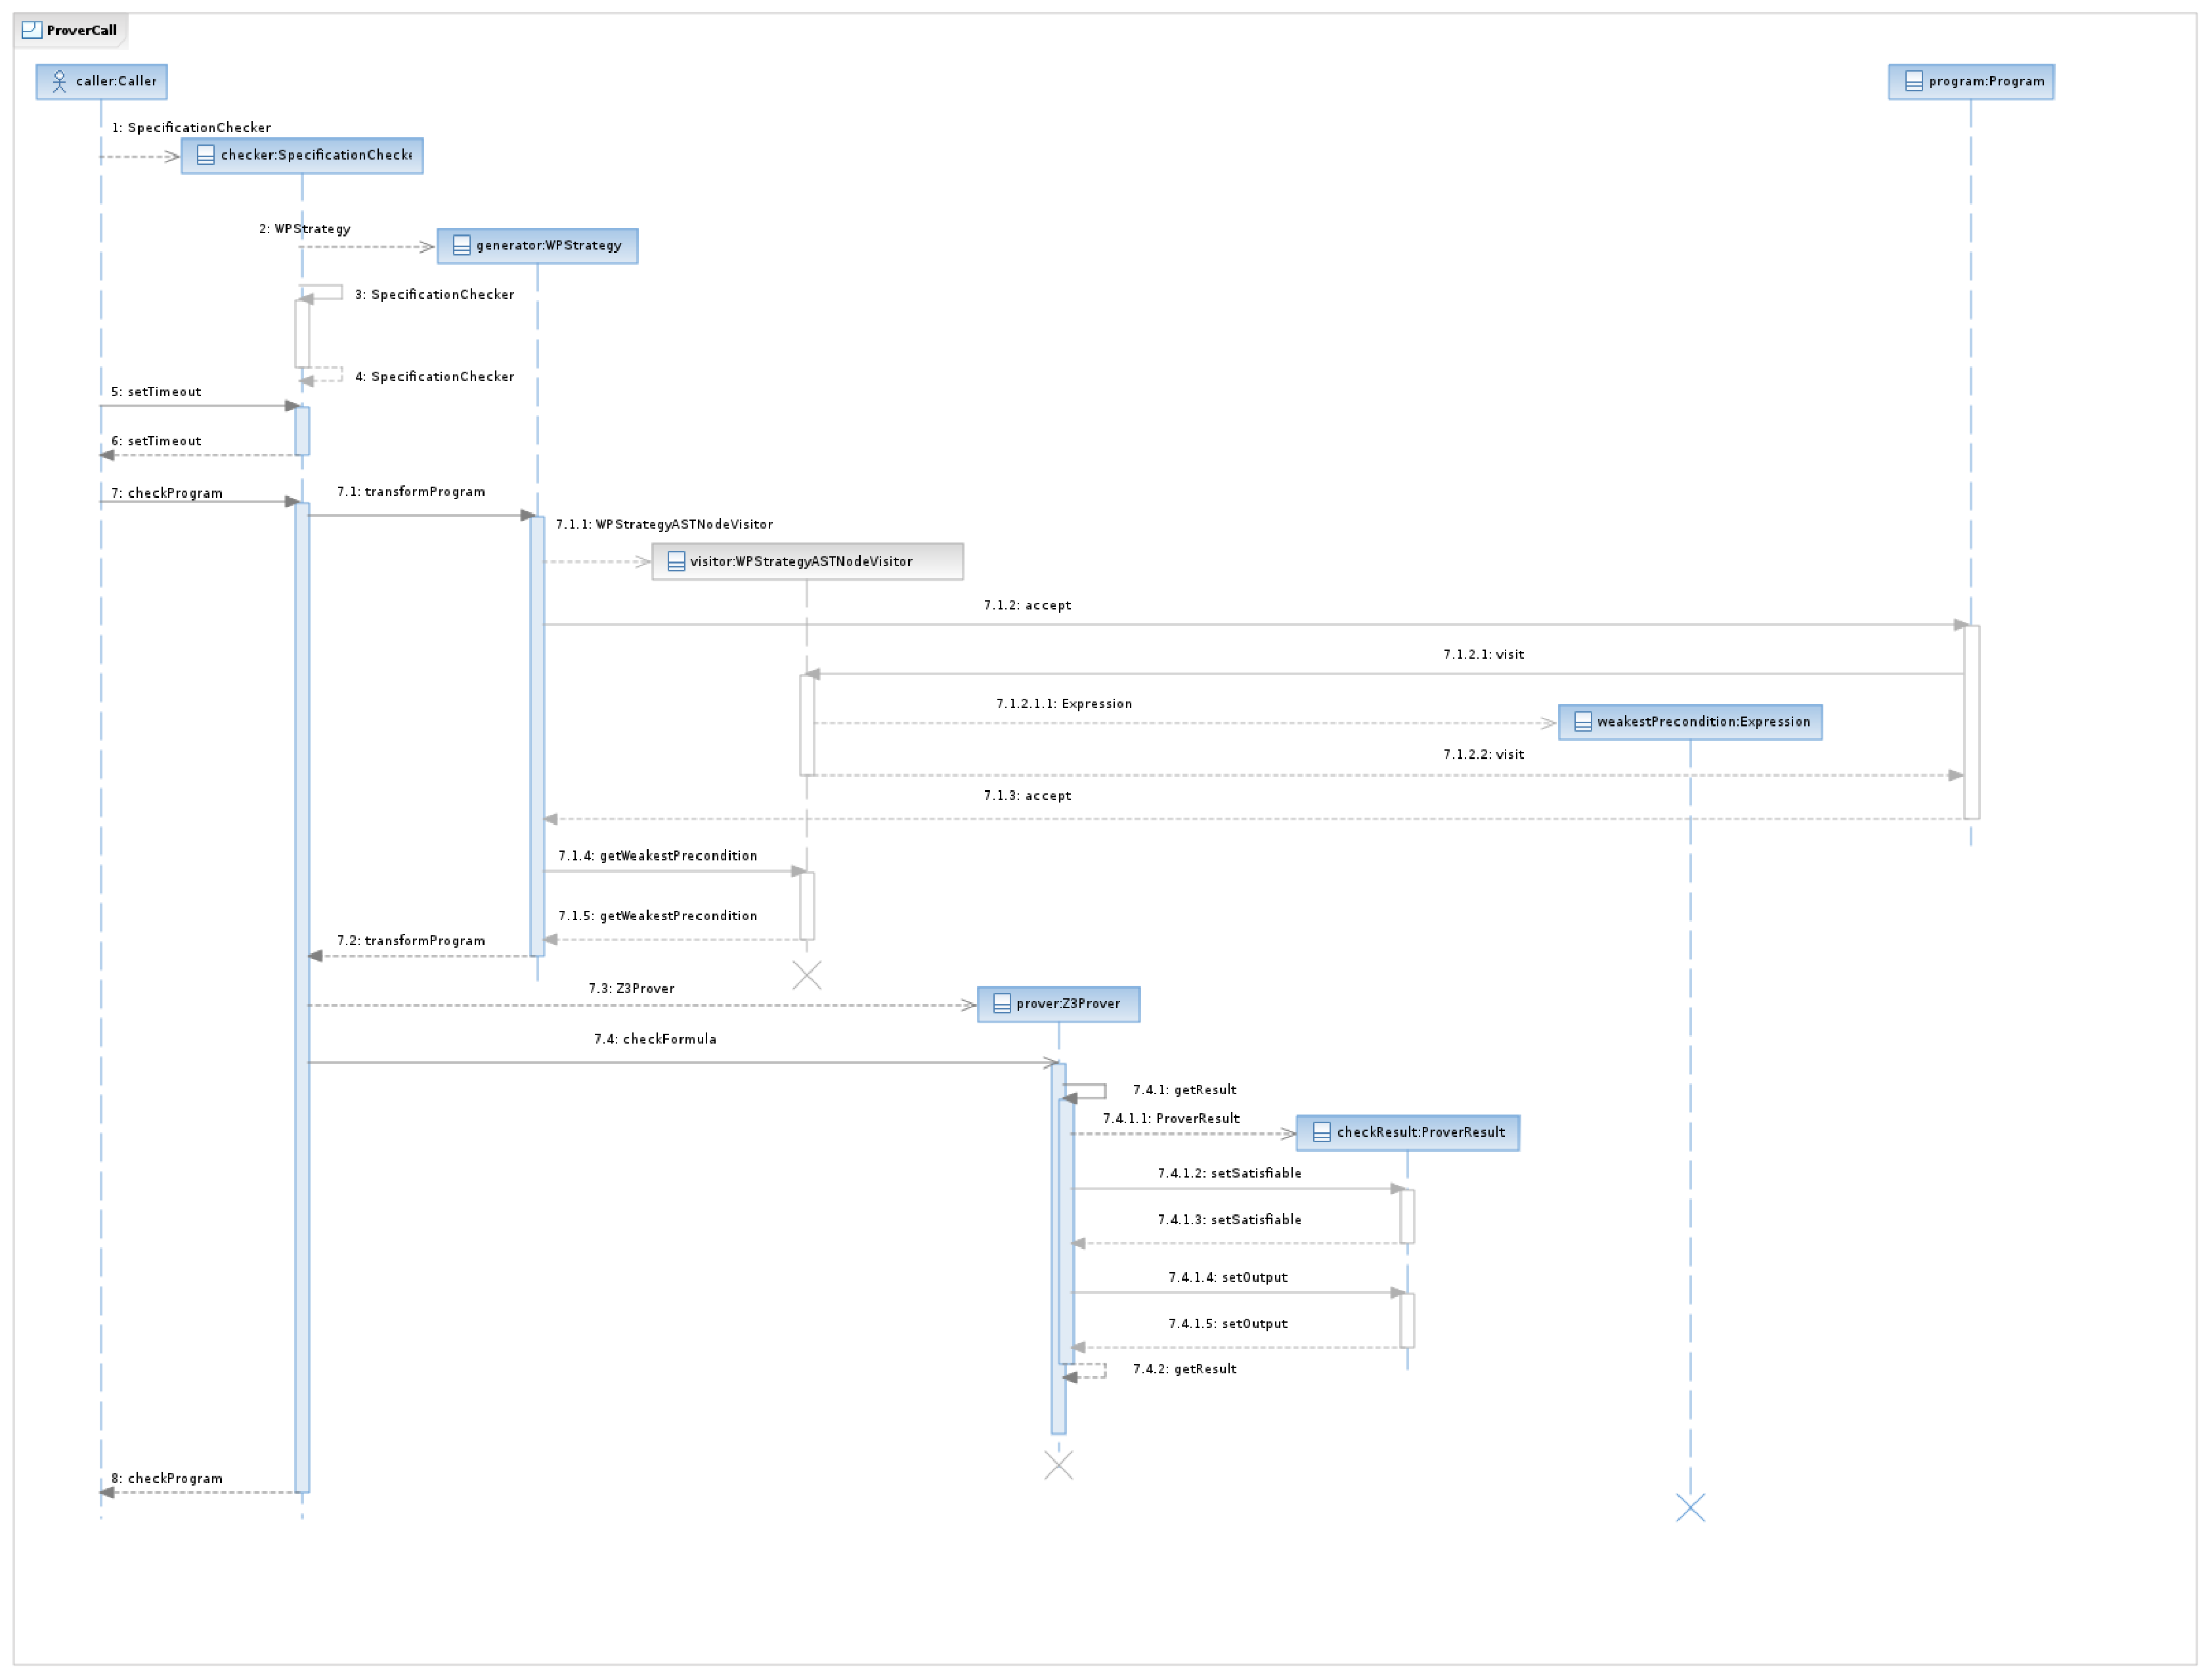
\includegraphics[height=1.2\textheight]{diagrams/programchecking_sequence.pdf}%

        \caption{Sequenzdiagramm zum Aufruf der Beweiserschnittstelle,
        um eine Programmspezifikation zu überprüfen.}%

        \label{programchecking_sequencediagram}%
    \end{figure}%
\end{landscape}%
